\documentclass{beamer}
%
% Choose how your presentation looks.
%
% For more themes, color themes and font themes, see:
% http://deic.uab.es/~iblanes/beamer_gallery/index_by_theme.html
%
\mode<presentation>
{
  \usetheme{CambridgeUS}      % or try Darmstadt, Madrid, Warsaw, ... CambridgeUS
  \usecolortheme{seahorse} % or try albatross, beaver, crane, ...
  \usefonttheme{serif}  % or try serif, structurebold, ...
  % \setbeamertemplate{navigation symbols}{}
  \setbeamertemplate{caption}[numbered]
  % \addtobeamertemplate{navigation symbols}{}{%
  %   \usebeamerfont{footline}%
  %   \usebeamercolor[fg]{footline}%
  %   \hspace{1em}%
  %   \insertframenumber/\inserttotalframenumber
% }
} 

\usepackage[english]{babel}
\usepackage[utf8x]{inputenc}

\usepackage{hyperref}
\usepackage{amsmath}
\usepackage{amsfonts}
\usepackage{amssymb}
\usepackage{graphicx}
\usepackage{nameref}
\usepackage{multicol}
\usepackage{float}
\usepackage{multirow}
\usepackage[ruled, linesnumbered]{algorithm2e}


% \numberwithin{equation}{subsection}
% \renewcommand{\thesubsection}{\thesection.\arabic{subsection}}
% \renewcommand{\thesubsubsection}{\Alph{subsubsection}}
% \newcommand{\setsubsubsectionnumber}[1]{\setcounter{subsubsection}{#1}\addtocounter{subsubsection}{-1}}

\newcommand{\abs}[1]{\vert #1\vert}
\newcommand{\tab}[1][30pt]{\hspace*{#1}}
\newcommand{\bracket}[1]{\biggl[#1\biggr]}
\newcommand{\norm}[1]{\left\lVert #1\right\rVert}


\DeclareMathOperator*{\argmin}{arg\,min}
\DeclareMathOperator*{\argmax}{arg\,max}
\DeclareMathOperator*{\divergance}{D}
\DeclareMathOperator*{\LDS}{LDS}
\DeclareMathOperator*{\sign}{sign}


\newcommand*{\D}[2]{\divergance \left[#1, #2\right]}



\title[Virtual Adversarial Training]{Virtual Adversarial Training: A Regularization Method for Supervised and Semi-Supervised Learning}
\author{Ali Abbasi}
\date{}

\begin{document}

\begin{frame}
\titlepage
\vspace{-0.8 in}
\begin{center}
Information Theory, Statatistics, and Learning\\
Prof. Yassaee\\
{\small Sharif University of Technology}
\end{center}
\end{frame}

\begin{frame}{Outline}
\tableofcontents
\end{frame}


\section{Introduction}

\begin{frame}{Adversarial Attacks}

\begin{enumerate}[$\Rightarrow$]
 \item Cause a machine learning model to make incorrect predictions.
  \item Achieved by perturbations that maximally degrade the information contained in an input signal.
  \pause
  \item Deep learning systems have been shown to be vulnerable to adversarial attacks
  \item Their outputs can be manipulated with imperceptibly small perturbations applied to the inputs
\end{enumerate}
\end{frame}

\begin{frame}{Adversarial Attacks}
\begin{figure}[H]
\centering
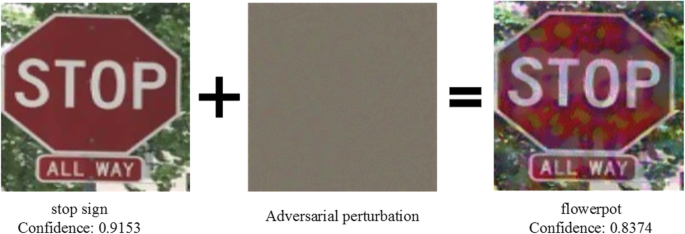
\includegraphics[width=0.8\columnwidth]{stop sign.png}
\end{figure}
\end{frame}

\begin{frame}{Optimal Adversarial Attacks}
% first paper
Some Notations:
\newline
U: the quantity (or label) of interest \newline
X: data generated from U \newline
\newline
Goal?\newline
Adding random perturbation E to X, producing random variable Y = X + E, such that the mutual information between U and Y = X + E is minimized
\pause 
\newline
\newline
NOTE: Since adding perturbations often introduces costs, we put constraints on the
perturbation E
\end{frame}

\begin{frame}{Optimal Adversarial Attacks}
the problem can be formulated as:
\begin{align*}
\min_{p(E|U,X)\in \mathcal{P}} I(U;X+E)
\end{align*}
where $\mathcal{P}$ is a set of admissible probability distributions.
\pause
\newline
for example, it can be:
\begin{align*}
\mathcal{P} &= \{p(E|U,X): \mathbb{E}[\norm{E}^2] \leq \epsilon, X \in \Omega\}
\end{align*}
\end{frame}

\begin{frame}{Robustness}
The property of a model to perform well and produce reliable results even when faced with unexpected or anomalous inputs
\newline 
\newline 
A robust loss (say, absolute error) may be preferred over a non-robust loss (say, squared error) due to its reduced sensitivity to large errors
\end{frame}

% TODO: connect robustness and regularization

\begin{frame}{Semi-Supervised Learning}
\begin{itemize}
    \item Labeling is hard, but there are often a lot of data
    \item Want to use unlabeled data to help training
\end{itemize}
\end{frame}

\begin{frame}{Regularization}
Adding a penalty term to the loss function \newline 
$\Rightarrow$  Discourages the model from having large weights for any of its features
\newline $\Rightarrow$ Prevent overfitting
\newline $\Rightarrow$ More robust to variations in the input data (Improve robustness)
\end{frame}

\begin{frame}{Regularization}
Can be interpreted as a prior distribution that reflects our educated a priori knowledge or belief regarding the model (from a Bayesian standpoint)
\pause 
\newline
\newline
A popular a priori belief $\rightarrow$ the outputs of systems are smooth with respect to spatial and/or temporal inputs
\end{frame}

%TOD


\section{Related Works}
\begin{frame}{Other Methods}
\begin{itemize}
  \item Label Propagation:
  \newline
  \newline
  Assign class labels to unlabeled training samples based on the belief that close input data points tend to have similar class labels
  \pause
  \newline
  \item Artificial Input:
  \newline
  \newline
Apply random perturbations to each input in order to generate artificial input points and encourage the model to assign similar outputs to the set of artificial inputs derived from the same point
\end{itemize}
\end{frame}
\begin{frame}{Other Methods}
\begin{enumerate}
  \item[?] But, what is the problem with these methods?
  \newline
  \newline
They often leave the predictor particularly vulnerable to a small perturbation in a specific direction called adversarial direction $\rightarrow$ it's the direction in the input
space in which the label probability $p(y = k|x)$ of the model
is most sensitive
\end{enumerate}
\end{frame}


\begin{frame}{Other Methods}
\begin{itemize}
\item  Contractive Loss:
\newline
\newline
Impose constraints on the Frobenius norm of the Jacobian matrix of the output with respect to the input
\newline 
\newline
 Deep Contractive Network, which imposes a layer-wise contraction penalty in a feed-forward neural network. The layer-wise penalty approximately minimizes the network outputs variance with respect to perturbations in the inputs, enabling the trained model to achieve “flatness” around the training data points.
\end{itemize}
\end{frame}

\begin{frame}{Other Methods}
\begin{enumerate}
  \item[?] But, what is the problem with this method?
  \newline
  \newline
  Computing the full Jacobian is computationally expensive and therefore they approximate it.
  \newline
  However, possibly because of their layer-wise approximation, their method was not successful in significantly decreasing the test error
%
\end{enumerate}
\end{frame}

\begin{frame}{Other Methods}
\begin{itemize}
\item  Generative adversarial networks (GANs)
\newline
\newline
Do not require an explicit definition of smoothness. 
\newline
\newline
Based on an objective function that trades off mutual information between observed examples and their predicted categorical class distribution, against the robustness of the classifier to an adversarial generative model. The resulting algorithm can be interpreted as a natural generalization of the generative adversarial networks (GAN) framework to robust classification against an optimal adversary.
\end{itemize}
\end{frame}

\begin{frame}{Other Methods}
\begin{enumerate}
  \item[?] But, what is the problem with this method?
  \newline
  \newline
In practice, these methods often require
careful tuning of many hyperparameters in the generative
model, and are usually not easy to implement without high
expertise in its optimization process.
\end{enumerate}
\end{frame}


\begin{frame}{Other Methods}
\begin{itemize}
  \item Adversarial Training:
  \newline 
  \newline
  Trains the model to assign to each input data a label that is similar to the labels to be assigned to its neighbors in the adversarial direction.
  \newline 
  Adversarial Direction $\rightarrow$ direction that can most greatly “deviate” the prediction of the model from the correct label.
\end{itemize}
\end{frame}

\begin{frame}{Other Methods}
\begin{enumerate}
  \item[?] But, what is the problem with this method?
  \newline
  \newline
Labeled data are needed for calculating the adversarial direction.
\end{enumerate}
\pause
\vspace{2em}
% \newline
% \hfill \break
% \hfill \break
Hence, the best method would be a method that considers Anisotropic smoothing and does not need labeled data to calculate the adversarial direction
\end{frame}

\section{Adversarial Training}
\begin{frame}{Some Notations}
I: Input dimension   \hfill  Q: Space of all labels
\newline
\newline
Input vector: $x\in R^{I}$ \hfill Output label: $y\in Q$
\newline
\newline
$p(y|x,\theta)$: Output distribution parameterized by $\theta$
\newline
\newline
$\hat{\theta}$: vector of the model parameters at a specific iteration step of the training process. 
\end{frame}

\begin{frame}{Some Notations}
Labeled Dataset: 
$\mathcal{D}_l = \{x_{l}^{n},y_{l}^{n}| n = 1,...,N_l\}$
\newline
\newline
Unlabeled Dataset:
$\mathcal{D}_{ul} = \{x_{ul}^{m}| m = 1,...,N_{ul}\}$
\end{frame}


\begin{frame}{Adversarial Training}
The loss function of adversarial training:
\\
\begin{align*}
L_{adv}(x_l, \theta) &= \D{q(y | x_l)}{p(y | x_l + r_{adv}, \theta)}\\
r_{adv} &= \argmax_{r; \norm{r} \le \epsilon} \D{q(y | x_l)}{p(y | x_l + r, \theta)}
\end{align*}
$D[p,p']$ :divergence between two distributions \(p\) and \(p'\)
\newline
$q(y|x_l)$ : true distribution of the output label, which is unknown.
\newline
\newline
Goal: approximate the true distribution by a parametric model $p(y|x_l,\theta)$ that is robust against adversarial attack to \(x\).
\end{frame}

\begin{frame}{Adversarial Training}
When the norm is $L_2$, adversarial perturbation can be approximated by:
\begin{align*}
r_{adv} &\approx \epsilon \frac{g}{\norm{g}_2}
\end{align*}
\begin{align*}
g = \nabla_{x_l} \D{h(y ; y_l)}{p(y | x_l, \theta)}\\
\end{align*}
\(g\) can be efficiently computed by backpropagation.
\newline
When the norm is $L_\infty$:
\begin{align*}
r_{adv} &\approx \epsilon \sign(g)
\end{align*}
\end{frame}


\section{Virtual Adversarial Training}
\begin{frame}{Virtual Adversarial Training}
Let \(x_*\) represent either a labeled (\(x_l\)) or unlabeled (\(x_{ul}\)) data point.
Our objective function is:
\begin{align*}
&\D{q(y | x_*)}{p(y | x_* + r_{qadv}, \theta)}\\
\text{Where: } &r_{qadv} = \argmax_{r; \norm{r} \le \epsilon} \D{q(y | x_*)}{p(y | x_* + r, \theta)}
\end{align*}
\pause
But we have no information about \(q(y | x_{ul})\).\\
\pause
We'll use its current estimate, \(p(y | x_*, \theta)\) instead (hence the term virtual).
\end{frame}

\begin{frame}{Virtual Adversarial Training}
We denote the current parameters as \(\hat{\theta}\). So the \textit{Local Distributional Smoothness} is defined as:
\begin{align*}
\LDS(x_*, \theta) &= \D{p(y | x_*, \hat{\theta})}{p(y | x_* + r_{vadv}, \theta)}\\
r_{vadv} &= \argmax_{r; \norm{r} \le \epsilon} \D{p(y | x_*, \hat{\theta})}{p(y | x_* + r, \theta)}
\end{align*}

\end{frame}


\begin{frame}{}
The regularization term proposed in the paper is simply the average of \(\LDS\) over all data points:
\begin{align*}
\mathcal{R}(\mathcal{D}_l, \mathcal{D}_{ul}, \theta) = \frac{1}{N_l + N_{ul}} \sum_{x_* \in \mathcal{D}_l, \mathcal{D}_{ul}} \LDS(x_*, \theta)
\end{align*}
    
And the full objective becomes:
\begin{align*}
\mathcal{L} = \ell(D_l, \theta) + \alpha \mathcal{R}(D_l, D_{ul}, \theta)
\end{align*}
\end{frame}

\section{Approximating Virtual Adversarial Direction}

\begin{frame}
\frametitle{Approximating \(r_{vadv}\)}
Assume twice differentiability of \(p(y|x_*, \theta)\) (and as a result \(\divergance\)) with respect to \(x_*\) and \(\theta\).
\(\divergance\) archives the minimum value at \(r = 0\):
\begin{align*}
\divergance(r, x, \hat{\theta})|_{r=0} = 0 \implies \nabla_r \divergance(r, x, \hat{\theta})|_{r=0} = 0
\end{align*}
\pause
The evaluation of \(r_{vadv}\) cannot be performed with the linear approximation as in the original adversarial training since the gradient of \(\divergance(r, x_*, \hat{\theta}) \triangleq\D{p(y | x_*, \hat{\theta})}{p(y | x_* + r, \theta)}\) with respect to \(r\) is always zero at \(r = 0\).
\end{frame}

\begin{frame}
\frametitle{Approximating \(r_{vadv}\)}
We can derive second order Taylor expansion of \(\divergance\) as follows:
\begin{align*}
\divergance(r, x, \hat{\theta}) \approx \frac{1}{2} r^T H(x, \hat{\theta})r
\end{align*}

Where \(H(x, \hat{\theta})\) is the Hessian matrix of \(\divergance\) with respect to \(r\).\\

\pause

We know that the maximum value of \(\divergance\) is achieved when \(r\) is the eigenvector \(u(x, \hat{\theta})\) of the matrix \(H\) corresponding to the largest eigenvalue:
\begin{align*}
r_{vadv} &\approx \argmax_r\left\{r^T H(x, \hat{\theta})r \mid \norm{r} \le \epsilon\right\}\\
&= \epsilon \overline{u(x, \hat{\theta})} \tag{\(\overline{v} = \frac{v}{\norm{v}}\)}
\end{align*}
\end{frame}

\begin{frame}
    \frametitle{Approximating \(r_{vadv}\)}
What about \(O(I^3)\) complexity of computing the eigenvector?

\pause
We use the iterative \textit{Power Method} to approximate the dominant eigenvector.
Suppose \(d\) is a random unit vector. If \(d\) is not prependicular to the dominant eigenvector, then iterative calculation of
\begin{align*}
d \leftarrow \overline{Hd}
\end{align*}
converges to the dominant eigenvector (see~\nameref{sec:appendix}).
\end{frame}

\begin{frame}
\frametitle{Approximating \(r_{vadv}\)}
We can approximate \(Hd\) with difference method too:
\begin{align*}
Hd &\approx \frac{\nabla_r \divergance(r, x_*, \hat{\theta})|_{r=\xi d} - \nabla_r \divergance(r, x_*, \hat{\theta})|_{r=0}}{\xi}\\
&= \frac{\nabla_r \divergance(r, x_*, \hat{\theta})|_{r=\xi d}}{\xi}
\end{align*}
\pause 
\begin{align*}
\implies d \leftarrow \overline{\nabla_r \divergance(r, x_*, \hat{\theta})|_{r=\xi d}}&&
\end{align*}
Thus, the approximation of \(r_{vadv}\) with \(K\) steps of the power method can be achieved with \(K\) sets of backpropagation.
\end{frame}

\begin{frame}
\frametitle{Approximation for Derivative of Regularization Term}
\begin{center}
\begin{minipage}{0.9\linewidth}
\begin{algorithm}[H]
\caption{Mini-batch SGD for \(\nabla_\theta\mathcal{R}\) with one time iteration of power method}
Choose \(M\) random samples from dataset \(\mathcal{D}\): \(\left\{x^{(i)}\right\}_{i=1}^M\).\\
Sample unit vector \(d^{(i)}\) from an iid Gaussian distribution.\\
Calculate \(r_{vadv}\) with one set of backpropagation:
\begin{align*}
g^{(i)} &\gets \left.\nabla_r \D{p(y | x^{(i)}, \hat{\theta})}{p(y | x^{(i)} + r, \theta)}\right|_{r=\xi d^{(i)}}\\
r_{vadv}^{(i)} &\gets \epsilon \frac{g^{(i)}}{\norm{g^{(i)}}}
\end{align*}\\
\Return{\(\nabla_\theta \left(\frac{1}{M}\sum_{i=1}^M \D{p(y | x^{(i)}, \hat{\theta})}{p(y | x^{(i)} + r_{adv}^{(i)}, \theta)}\right)\)}
\end{algorithm}
\end{minipage}
\end{center}
\end{frame}

\subsection{Tuning Hyperparameters}
\begin{frame}
    \frametitle{Tuning Hyperparameters}

We have two hyperparameters: \(\epsilon\) and \(\alpha\).

\begin{align*}
\max_r\left\{ \divergance(r, x, \theta) \mid \norm{r}_2 \le \epsilon\right\} & \approx \max_r\left\{\frac{1}{2} r^T H(x, \theta)r \mid \norm{r}_2 \le \epsilon\right\}\\
& = \frac{1}{2} \epsilon^2 \lambda_1(x, \theta)
\end{align*}
    
\pause
\begin{align*}
\mathcal{L} &= \ell(\theta, \mathcal{D}_l) + \alpha \mathcal{R}_{vadv} (\theta, \mathcal{D}_l, \mathcal{D}_{ul})\\
&= \ell(\theta, \mathcal{D}_l) + \alpha \frac{1}{N_l + N_{ul}} \sum_{x \in \mathcal{D}_l, \mathcal{D}_{ul}} \max_r\left\{ \divergance(r, x, \theta) \mid \norm{r}_2 \le \epsilon\right\}\\
& \approx \ell(\theta, \mathcal{D}_l) + \frac{1}{2} \epsilon^2\alpha \frac{1}{N_l + N_{ul}} \sum_{x \in \mathcal{D}_l, \mathcal{D}_{ul}}  \lambda_1(x, \theta)
\end{align*}

\end{frame}

\section{Experiments}

\begin{frame}
    \frametitle{Experiments}
\begin{align*}
\divergance =& \text{KL Divergence}\\
\xi =& 10^{-6}\\
\alpha =& 1\\
\text{Model} =& \text{Simple Fully Connected Network with 4 hidden layers}\\&\text{ for MNIST and Conv-Large for CIFAR-10}
\end{align*}
\end{frame}

\begin{frame}
    \frametitle{Experiments}
\begin{table}
\centering
\caption{Test performance of supervised learning methods
on MNIST with 60,000 labeled examples in the permutation
invariant setting.}
\label{tab:mnist}
\begin{tabular}{l r}
\hline
\hline
Method & Test error rate(\%)\\
\hline
SVM (Gaussian kernel) & 1.40\\
Dropout  & 1.05\\
Adversarial, \(L_\infty\) norm constraint &  0.78\\
Ladder networks &  0.57 (\(\pm\)0.02)\\
\hline
Baseline (MLE) & 1.11 (\(\pm\)0.06)\\
RPT & 0.84 (\(\pm\)0.03)\\
Adversarial, \(L_1\) norm constraint &0.79 (\(\pm\)0.03)\\
Adversarial, \(L_2\) norm constraint& 0.71 (\(\pm\)0.03)\\
VAT &0.64 (\(\pm\)0.05)\\
\hline
\hline
\end{tabular}
\end{table}
\end{frame}

\begin{frame}
    \frametitle{Experiments}

\begin{table}
\centering
\caption{Test performance of supervised learning methods
implemented with CNN on CIFAR-10 with 50,000 labeled
examples.}
\label{tab:ciphar10}
\begin{tabular}{l r}
\hline
\hline
Network in Network & 8.81\\
All-CNN & 7.25\\
Deeply Supervised Net & 7.97\\
Highway Network & 7.72\\
ResNet (1001 layers) & 4.62 (\(\pm\)0.20)\\
DenseNet (190 layers) & 3.46\\
\hline
Baseline (only with dropout) &6.67 (\(\pm\)0.07)\\
RPT &6.30 (\(\pm\)0.04)\\
VAT &5.81 (\(\pm\)0.02)\\
\hline
\hline
\end{tabular}
\end{table}

\end{frame}


\begin{frame}
\frametitle{Experiments}
\vspace{-1em}
\begin{table}
\centering
\caption{Test performance of semi-supervised learning
methods.}
\label{tab:semi}
\resizebox{0.75\columnwidth}{!}{%
\begin{tabular}{l r r}
\hline
\hline
\multirow{3}{*}{Method} & \multicolumn{2}{c}{Test error rate(\%)}\\
& SVHN & CIFAR-10 \\
& \(N_l = 1000\) & \( N_l = 4000\)\\
\hline
SWWAE & 23.56&\\
% *Auxiliary DGM & 22.86&\\
% *Skip DGM & 16.61 (\(\pm\)0.24)&\\
Auxiliary DGM & 22.86&\\
Skip DGM & 16.61 (\(\pm\)0.24)&\\
Ladder networks, \(\Pi\) model && 20.40 (\(\pm\)0.47)\\
CatGAN && 19.58 (\(\pm\)0.58)\\
GQAN with FM & 8.11 (\(\pm\)1.3) &18.63 (\(\pm\)2.32)\\
model & 5.43 (\(\pm\)0.25) &16.55 (\(\pm\)0.29)\\
\hline
(on Conv-Small) & & \\
RPT & 8.41 (\(\pm\)0.24) & 18.56 (\(\pm\)0.29)\\
VAT & 6.83 (\(\pm\)0.24) & 14.87 (\(\pm\)0.13)\\
\hline
(on Conv-Large) & & \\
VAT & 5.77 (\(\pm\)0.32) & 14.18 (\(\pm\)0.38)\\
VAT+EntMin & 4.28 (\(\pm\)0.10)  & 13.15 (\(\pm\)0.21)\\
\hline
\hline
\end{tabular}%
}
\end{table}
\end{frame}

\begin{frame}
    \frametitle{Conditional Entropy Minimization}
VAT + \underline{EntMin}:
\begin{align*}
\mathcal{R}_{cent} &= \mathcal{H}(Y|X)\\
&= -\frac{1}{N_l + N_{ul}} \sum_{x\in \mathcal{D}_l, \mathcal{D}_{ul}}\sum_{y} p(y|x, \theta) \log p(y|x, \theta)
\end{align*}
\end{frame}

\begin{frame}
\frametitle{Performance of VAT with different \(\epsilon\)}
\begin{figure}
\centering
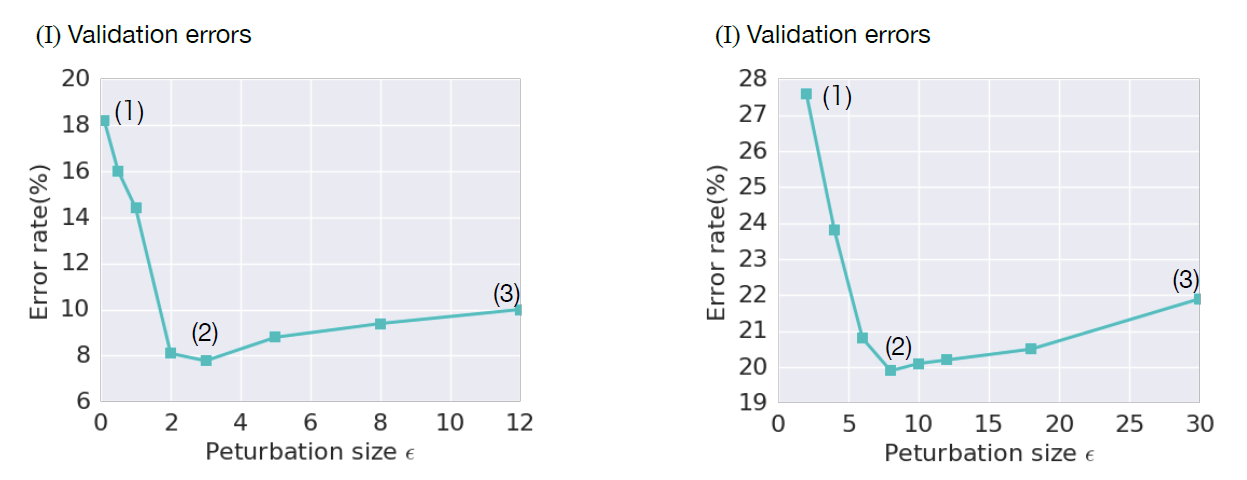
\includegraphics[width=0.8\columnwidth]{different_eps_val.png}
\caption{Validation error rate of VAT with different \(\epsilon\) on SVHN and CIFAR-10.}
\label{fig:different_eps_val}
\end{figure}
\end{frame}

\begin{frame}
\frametitle{Performance of VAT with different \(\epsilon\)}
\begin{figure}
\centering
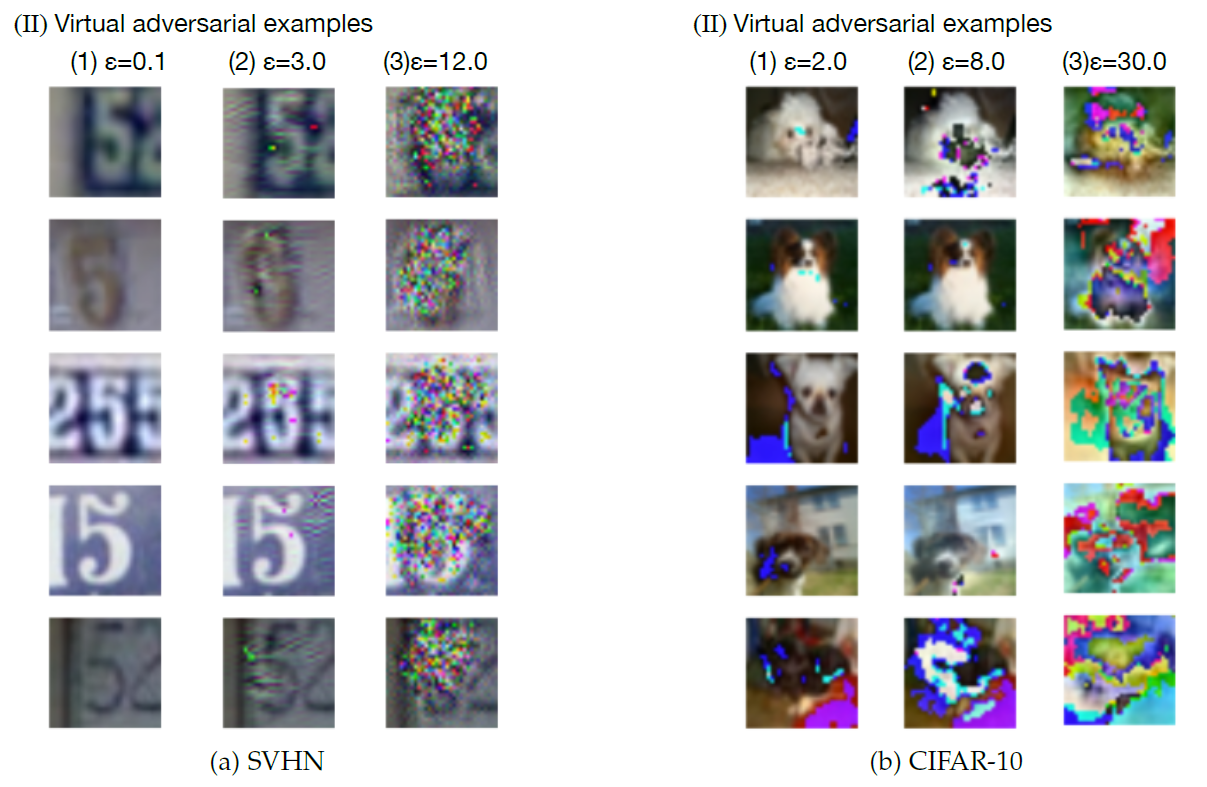
\includegraphics[width=0.8\columnwidth]{different_eps_images.png}
\caption{Images distorted with \(r_{vadv}\) with different \(\epsilon\) on SVHN and CIFAR-10.}
\label{fig:different_eps_images}
\end{figure}
\end{frame}

\begin{frame}
\frametitle{Conclusion}
\begin{itemize}
\item Effective model for both supervised and semi-supervised learning on different datasets
\item Small computational cost
\item Model agnostic
\item Simple:
\begin{itemize}
\item Requires optimization of only one hyperparameter
\item Does not require training of additional models
\end{itemize}
\end{itemize}

\end{frame}
\section{Question and Answer}
\begin{frame}{Thank You!}

Thanks for your attention :)

\begin{figure}[H]
\centering

\includegraphics[width=0.8\columnwidth]{meme.jpg}
\end{figure}
\vspace{1em}
\begin{center}
Any questions?
\end{center}
\end{frame}

\section{References}
\begin{frame}{References}
\begin{enumerate}
    \item Takeru Miyato, Shin-ichi Maeda, Masanori Koyama, Shin Ishii. ``Virtual Adversarial Training: A Regularization Method for Supervised and Semi-Supervised Learning", 2018.
    \item Jirong Yi, Raghu Mudumbai and Weiyu Xu. ``Derivation of Information-Theoretically Optimal Adversarial Attacks with Applications to Robust Machine Learning", 2020.
    \item Shixiang Gu, Luca Rigazio. ``Towards deep neural network architectures robust to adversarial examples", 2015.
    \item Jost Tobias Springenberg, ``Unsupervised and semi-supervised learning with categorical generative adversarial networks", 2015.
    \item Yves Grandvalet, Yoshua Bengio. ``Semi-supervised learning by entropy minimization", NIPS, 2004.
\end{enumerate}
\end{frame}
\section{Appendix}
\label{sec:appendix}

\begin{frame}
    \frametitle{Power Method}

We want to find the dominant eigenvector of the matrix \(A\) with eigenvectors \(v_1, v_2, \ldots, v_n\) sorted in descending order of their eigenvalues.\\
We will show that the iterative method \(d_{t+1} = A d_t
\) will converge to a multiple of the dominant eigenvector \(v_1\) provided that \(d_0\) is not orthogonal to \(v_1\).\\
\begin{align*}
\text{Suppose } d_0 &= c_1 v_1 + c_2 v_2 + \cdots + c_n v_n\\
\implies d_k &= Ad_{k-1} = A^k d_0 = A^k (c_1 v_1 + A^k c_2 v_2 + \cdots + A^k c_n v_n)\\
&= \lambda_1^k c_1 v_1 + \lambda_2^k c_2 v_2 + \cdots + \lambda_n^k c_n v_n\\
&= \lambda_1^k (c_1 v_1 + \left(\frac{\lambda_2}{\lambda_1}\right)^k c_2 v_2 + \cdots + \left(\frac{\lambda_n}{\lambda_1}\right)^k c_n v_n)\\
&\xrightarrow[]{k \to \infty} \lambda_1^k c_1 v_1
\end{align*}
\end{frame}

\end{document}
